\documentclass[a4paper, 11pt]{article}
\usepackage{hyperref}
\usepackage[margin=0.5in]{geometry}

\usepackage{amsmath}
\usepackage[arrowdel]{physics}
\usepackage{tensor}

\newcommand{\lag}{\ensuremath{\mathcal{L}}}
\newcommand{\p}{^{\prime}}
\newcommand{\ub}[1]{\vb{e}_{#1}}
\newcommand{\trcou}[2]{\tensor{\Lambda}{^{#1}_{#2}}}
\newcommand{\trcod}[2]{\tensor{\Lambda}{_{#1}^{#2}}}
\newcommand{\kdelta}[2]{\tensor*{\delta}{^{#1}_{#2}}}
\newcommand{\del}[3][]{\partial^{#1}_{#2}#3}
\newcommand{\integ}[5][]{\int\limits_{#2}^{#3}\dd[#1]{#4}#5}

\title{Summary of SI2371 Special Relativity}
\author{Yashar Honarmandi \\ yasharh@kth.se}
\date{\today}

\begin{document}

\maketitle

\begin{abstract}
	Detta ær en sammanfattning av kursen SH1014 Modern fysik.
\end{abstract}

\pagenumbering{roman}
\thispagestyle{empty}

\newpage

\tableofcontents

\newpage

\pagenumbering{arabic}

\section{Basic Concepts}

\paragraph{The Classical Hall Effect}
Consider a slab of some conducting material. In the simple kinetic theory of electrons in a conductor the equation of motion is
\begin{align*}
	\expval{\dv{\vb{v}}{t}} + \frac{1}{\tau}\expval{\vb{v}} = \frac{1}{m}\vb{F}.
\end{align*}
Suppose now that the slab were to be immersed in an electric field $E\vb{e}_{x}$ and a magnetic field $B\vb{e}_{z}$. In the steady state we have
\begin{align*}
	\frac{1}{\tau}\expval{\vb{v}} = -\frac{e}{m}\left(\left(E + v_{y}B\right)\vb{e}_{x} + \left(E_{y} - v_{x}B\right)\vb{e}_{y}\right).
\end{align*}
We impose boundary conditions such that there is no net current flow in the $y$ direction. In the case of $B = 0$ we then find the conductivity $\sigma = \frac{ne^{2}\tau}{m}$. This will naturally also be the case for non-zero $B$ as $v_{y} = 0$ in the steady state. This also means that $v_{x} = -\frac{e\tau}{m}E$, and we find
\begin{align*}
	E_{y} = -\frac{e\tau}{m}EB.
\end{align*}
The steady-state current is now
\begin{align*}
	\vb{J} = -ne\expval{\vb{v}} = \frac{ne^{2}\tau}{m}\vb{E}.
\end{align*}
On tensor form we have
\begin{align*}
	E_{i} = \tensor{\rho}{_{i}^{j}}J_{j}.
\end{align*}
Evidently the resistivity tensor has diagonal components $\frac{1}{\sigma} = \frac{m}{ne^{2}\tau}$, but the addition of the magnetic field also provides an off-diagonal component
\begin{align*}
	\tensor{\rho}{_{y}^{x}} = -\frac{B}{ne}.
\end{align*}
This phenomenon is termed Hall resistance or the Hall effect. From this we define the Hall coefficient
\begin{align*}
	R_{\text{H}} = \frac{\tensor{\rho}{_{y}^{x}}}{B} = -\frac{1}{ne}.
\end{align*}

\paragraph{Failures of the Hall Effect}
The predictions based on these calculations turned out to give correct predictions for many materials, but some materials exhibited a reverse Hall effect in having a positive Hall coefficient, a property unexplainable by these purely classical arguments. The key point here is the assumption that the charge carriers have negative charge, an assumption which turns out to not be true in all materials.

\paragraph{The Bloch Theorem}
The full Hamiltonian for a set of electrons in a crystal lattice is impossible to solve. Bloch's theorem is the statement that by simplifying the theory such that the electrons are moving in some effective potential, the states are given by
\begin{align*}
	\braket{\vb{r}}{\vb{k}} = u(\vb{r})e^{i\vb{k}\cdot\vb{r}},
\end{align*}
where $u$ has the same periodicity as the potential.

\paragraph{The Tight Binding Approximation}
The tight binding approximation is an approximative solution of the Schrödinger equation in  a periodic potential. It states that, given some solution of one element of the periodic potential, the full state is a superposition of solutions localized at each element in the periodic array. More specifically, it is the approximation
\begin{align*}
	\ket{\psi_{\vb{q}}} = \frac{1}{\sqrt{N}}\sum\limits_{j}e^{i\vb{q}\cdot\vb{R}_{j}}\ket{j},
\end{align*}
with the corresponding Bloch function
\begin{align*}
	u_{\vb{q}}(\vb{r}) = \frac{1}{\sqrt{N}}\sum\limits_{j}e^{-i\vb{q}\cdot(\vb{r} - \vb{R}_{j})}\phi_{0}(\vb{r} - \vb{R}_{j}),
\end{align*}
where
\begin{align*}
	\phi_{0}(\vb{r} - \vb{R}_{j}) = \braket{\vb{r}}{j}.
\end{align*}

To compute the energy of such states we will need inner products of these states. First we have
\begin{align*}
	\braket{\psi_{\vb{q}}} = \frac{1}{N}\sum\limits_{j, l}e^{i\vb{q}\cdot(\vb{R}_{j} - \vb{R}_{l})}\braket{l}{j} = \sum\limits_{j}e^{i\vb{q}\cdot\vb{R}_{j}}\braket{0}{j},
\end{align*}
which we dub $\eta(\vb{q})$. Now, because these states are eigenstates of the translation operator one can show that
\begin{align*}
	\braket{\psi_{\vb{q}}}{\psi_{\vb{k}}} = \eta(\vb{q})\delta^{3}(\vb{q} - \vb{k})_{\vb{G}},
\end{align*}
where the Dirac delta is up to a reciprocal lattice vector. Next, let us consider matrix elements of the Hamiltonian. Writing
\begin{align*}
	\ham = \frac{p^{2}}{2m} + \sum\limits_{j}V(\vb{r} - \vb{R}_{j})
\end{align*}
we have
\begin{align*}
	\ham\ket{i} = E_{0}\ket{i} + \left(\sum\limits_{j\neq i}V(\vb{r} - \vb{R}_{j})\right)\ket{i}.
\end{align*}
Denoting the operator in the last term as $\Delta V_{i}$ we note that it does not have $\ket{i}$ as an eigenvector. For a Bloch state we then find
\begin{align*}
	\mel{\psi_{\vb{q}}}{\ham}{\psi_{\vb{q}}} = E_{0}\eta(\vb{q}) + \frac{1}{N}\sum\limits_{j, k}e^{i\vb{q}\cdot(\vb{R}_{k} - \vb{R}_{j})}\mel{j}{\Delta V_{k}}{k}.
\end{align*}
Defining the right term as $\Lambda(\vb{q})$ we find
\begin{align*}
	E_{\vb{q}} = E_{0} + \frac{\Lambda(\vb{q})}{\eta(\vb{q})}.
\end{align*}

Approximating the atoms to be far apart we can neglect most contributions to $\eta$ by setting it to $1$. In this approximation we introduce a first non-trivial correction by first setting
\begin{align*}
	\braket{j}{k} = \zeta
\end{align*}
and
\begin{align*}
	\expval{\Delta V_{k}}{k} = \Delta E,\ \mel{j}{\Delta V_{k}}{k} = t_{0},
\end{align*}
where the off-diagonal expressions only hold for nearest neighbors. $t_{0}$ is called the transfer integral. We then have
\begin{align*}
	\Lambda(\vb{q}) = \Delta E + t_{0}\sum\limits_{\vb*{\delta}}e^{-i\vb{q}\cdot\vb*{\delta}},
\end{align*}
where the sum is over nearest-neighbor lattice vectors. A similar result holds for the overlap. We often normalize the term by extracting a factor $z$ from the sum, which is the coordination number, and write what is left as $\gamma(\vb{q})$. We then finally have
\begin{align*}
	E_{\vb{q}} = E_{0} + \frac{\Delta E + t_{0}z\gamma(\vb{q})}{1 + z\zeta\gamma(\vb{q})}.
\end{align*}
Evidently, then, the band width is $2t_{0}z$. Furthermore, we can use this to determine the curvature and thus an effective mass by expanding
\begin{align*}
	E_{\vb{q}} \approx E_{0} + \frac{\hbar^{2}}{2m}\vb{q}^{2}
\end{align*}
close to the minimum.

\paragraph{Wannier Functions}
Wannier functions are constructions of states that are orthogonal. For band $n$, the Wannier function centered around atom $j$ is
\begin{align*}
	\ket{\chi_{n, j}} = \frac{1}{\sqrt{N}}\sum\limits_{\vb{q}}e^{-i\vb{q}\cdot\vb{R}_{j}}\ket{\psi_{n, \vb{q}}}.
\end{align*}
The $\ket{\psi_{n, \vb{q}}}$ are the normalized Bloch states from the tight binding approximation. These distinguish themselves in being useful even if the tight binding approximation breaks down.

\paragraph{Graphene}
Graphene is a phase of carbon where it forms a single atomic layer with the atoms arranged in a honeycomb lattice. This can be represented as a triangular lattice with two atoms in the basis. We choose the lattice vectors $a\left(\frac{3}{2}, \pm\frac{\sqrt{3}}{2}\right)$ and the basis displacement vector $a(1, 0)$. Employing the tight-binding approximation with $E_{0} = 0$ we write the Hamiltonian as
\begin{align*}
	\ham = -t\sum\limits_{\expval{i, j}}\op{i}{j} + \op{j}{i},
\end{align*}
which is a sum over nearest neighbors. The fact that there are two atoms in the basis divides the lattice into two sublattices $A$ and $B$. The Bloch states are then
\begin{align*}
	\ket{\vb{q}, A} = \frac{1}{\sqrt{N}}\sum\limits_{j\in A}e^{i\vb{q}\cdot\vb{R}_{j}}\ket{j},
\end{align*}
with a similar state for the other sublattice. Neglecting overlap between neighboring wavefunctions we find
\begin{align*}
	\ham\ket{\vb{q}, A} =& -\frac{t}{\sqrt{N}}\left(\sum\limits_{\expval{i, j}}\op{i}{j} + \op{j}{i}\right)\sum\limits_{k\in A}e^{i\vb{q}\cdot\vb{R}_{k}}\ket{k} \\
	                    =& -\frac{t}{\sqrt{N}}\sum\limits_{k\in A}\sum\limits_{j = \text{nn}(k)}e^{i\vb{q}\cdot\vb{R}_{k}}\ket{j} \\
	                    =& -\frac{t}{\sqrt{N}}\sum\limits_{k\in A}\sum\limits_{j = \text{nn}(k)}e^{i\vb{q}\cdot(\vb{R}_{j} - \vb*{\delta}_{k\to j})}\ket{j} \\
	                    =& -t\sum\limits_{\vb*{\delta}}e^{-i\vb{q}\cdot\vb*{\delta}}\ket{\vb{q}, B},
\end{align*}
and similarly
\begin{align*}
	\ham\ket{\vb{q}, B} =& -t\sum\limits_{\vb*{\delta}}e^{i\vb{q}\cdot\vb*{\delta}}\ket{\vb{q}, A}.
\end{align*}
We denote the prefactor as $-tf(\vb{q})$, and find that the Hamiltonian has eigenvalues $\pm t\abs{f(\vb{q})}$.

Of note about the Brillouin zone of the triangular lattice, which is a hexagon, is that it only has one unique corner (and its opposite), as the others are related to these by a reciprocal lattice vector. Choosing, say, $\vb{K} = \frac{4\pi}{3\sqrt{3}a}\left(\frac{\sqrt{3}}{2}, \frac{1}{2}\right)$ and its opposite we have
\begin{align*}
	f(\vb{K}) = e^{i\frac{4\pi}{3\sqrt{3}}\frac{\sqrt{3}}{2}} + e^{i\frac{4\pi}{3\sqrt{3}}\left(-\frac{\sqrt{3}}{4} - \frac{\sqrt{3}}{4}\right)} + e^{i\frac{4\pi}{3\sqrt{3}}\left(-\frac{\sqrt{3}}{4} + \frac{\sqrt{3}}{4}\right)} = 2\cos(\frac{2\pi}{3}) + 1 = 0.
\end{align*}
Thus there is no band gap. Next we have
\begin{align*}
	\grad_{\vb{q}}f(\vb{q}) = i\sum\limits_{\vb*{\delta}}\vb*{\delta}e^{i\vb{q}\cdot\vb*{\delta}},
\end{align*}
and close to the corner we have
\begin{align*}
	f(\vb{q}) \approx& (\vb{q} - \vb{K})\cdot ia\left((1, 0)e^{i\frac{2\pi}{3}} + \left(-\frac{1}{2}, -\frac{\sqrt{3}}{2}\right)e^{-i\frac{2\pi}{3}} + \left(-\frac{1}{2}, \frac{\sqrt{3}}{2}\right)\right) \\
	                =& ia\left(k_{x}e^{i\frac{2\pi}{3}} + \left(-\frac{1}{2}k_{x} - \frac{\sqrt{3}}{2}k_{y}\right)e^{-i\frac{2\pi}{3}} - \frac{1}{2}k_{x} + \frac{\sqrt{3}}{2}k_{y}\right) \\
	                =& ia\left(k_{x}\left(e^{i\frac{2\pi}{3}} - \frac{1}{2}e^{-i\frac{2\pi}{3}} - \frac{1}{2}\right) + k_{y}\left(-\frac{\sqrt{3}}{2}e^{-i\frac{2\pi}{3}} + \frac{\sqrt{3}}{2}\right)\right).
\end{align*}
This means that the dispersion is linear, a characteristic of solutions of the Dirac equation. This relation must be investigated further.

To do this we must remedy the fact that $f$ does not share the periodicity of the reciprocal lattice due to the $\vb*{\delta}$ not being lattice vectors. However, by introducing
\begin{align*}
	\ket{\vb{q}, \tilde{B}} = ie^{-i\vb{q}\cdot\vb*{\delta}_{1}}\ket{\vb{q}, B},
\end{align*}
the same treatment results in the Hamiltonian containing a new function $\tilde{f}(\vb{q}) = ie^{-i\vb{q}\cdot\vb*{\delta}_{1}}f(\vb{q})$. This function has the periodicity of the reciprocal lattice. Writing
\begin{align*}
	\tilde{f}(\vb{q}) = i\left(1 + e^{i\vb{q}\cdot\sqrt{3}a\left(-\frac{\sqrt{3}}{2}, \frac{1}{2}\right)} + e^{i\vb{q}\cdot\sqrt{3}a\left(-\frac{\sqrt{3}}{2}, -\frac{1}{2}\right)}\right),
\end{align*}
we have
\begin{align*}
	\grad_{\vb{q}}\tilde{f} =& -\sqrt{3}a\left(\left(-\frac{\sqrt{3}}{2}, \frac{1}{2}\right)e^{i\vb{q}\cdot\sqrt{3}a\left(-\frac{\sqrt{3}}{2}, \frac{1}{2}\right)} + \left(-\frac{\sqrt{3}}{2}, -\frac{1}{2}\right)e^{i\vb{q}\cdot\sqrt{3}a\left(-\frac{\sqrt{3}}{2}, -\frac{1}{2}\right)}\right).
\end{align*}
As $\tilde{f}(\vb{K}) = 0$ we have
\begin{align*}
	\tilde{f}(\vb{K} + \vb{k}) \approx& -\sqrt{3}a\left(\left(-\frac{\sqrt{3}}{2}, \frac{1}{2}\right)e^{i\frac{4\pi}{3}\left(-\frac{3}{4} + \frac{1}{4}\right)} + \left(-\frac{\sqrt{3}}{2}, -\frac{1}{2}\right)e^{i\frac{4\pi}{3}\left(-\frac{3}{4} - \frac{1}{4}\right)}\right)\cdot\vb{k} \\
	=& -\sqrt{3}a\left(\left(-\frac{\sqrt{3}}{2}, \frac{1}{2}\right)e^{-i\frac{2\pi}{3}} + \left(-\frac{\sqrt{3}}{2}, -\frac{1}{2}\right)e^{-i\frac{4\pi}{3}}\right)\cdot\vb{k} \\
	=& -\sqrt{3}a\left(-\frac{\sqrt{3}}{2}\left(e^{-i\frac{2\pi}{3}} + e^{-i\frac{4\pi}{3}}\right), \frac{1}{2}\left(e^{-i\frac{2\pi}{3}} - e^{-i\frac{4\pi}{3}}\right)\right)\cdot\vb{k} \\
	=& -\sqrt{3}a\left(-\sqrt{3}\cos(-\frac{2\pi}{3}), i\sin(-\frac{2\pi}{3})\right)\cdot\vb{k} \\
	=& -\frac{3}{2}a\left(1, -i\right)\cdot\vb{k}.
\end{align*}
In the matrix form we can represent the Hamiltonian in this basis as
\begin{align*}
	\tilde{\ham} = \frac{3}{2}at\mqty[
		0               & k_{x} - ik_{y} \\
		k_{x} + ik_{y}  & 0 \\
	] = v_{\text{F}}\vb*{\sigma}\cdot\vb{k}.
\end{align*}
This is an effective Hamiltonian for states close to the Brillouin zone boundary which is exactly the Dirac Hamiltonian in two dimensions. Doing the same around $-\vb{K}$ the Hamiltonian is $\tilde{\ham} = v_{\text{F}}(-\sigma_{x}k_{x} + \sigma_{y}k_{y})$. We can write this in a unified way by introducing a so-called valley degree-of-freedom index $\tau_{z} = \pm 1$.

\section{$4$-Vector Formalism}

$4$-vector formalism makes more explicit use of invariance relations that have previously been identified, most importantly the invariance of $c$, or so-called Lorentz invariance.

\paragraph{The Lorentz Group}
Consider a light pulse sent out from the origin at $t = 0$. The wavefront in the rest frame of the emitter satisfies $r^{2} = (ct)^{2}$. Next, for any frame in the standard configuration we must also have $(r\p)^{2} = (ct\p)^{2}$, implying the invariance of the quantity
\begin{align*}
	(ct)^{2} - r^{2}
\end{align*}
under any transformation that preserves the laws of physics. The Lorentz group is defined as the group of linear transforms that preserves the above quantity (linearity is to preserve important physical properties such as isotropy of space).

\paragraph{The Lorentz Boost in Matrix Form}
The Lorentz boost may now be written as
\begin{align*}
	\Lambda =
	\mqty[
		A & 0 \\
		0 & 1
	],\ 
	A =
	\mqty[
		\gamma       & -\beta\gamma \\
		-\beta\gamma & \gamma
	]
\end{align*}
such that $(x\p)^{\mu} = \tensor{\Lambda}{^{\mu}_{\nu}}x^{\nu}$, with Einstein summation from $0$ to $3$. This is also the general notation for Lorentz transformations, where $\Lambda$ may now be taken to be any element in the Lorentz group.

\paragraph{The Lorentz Group}
The Lorentz group is the group of all linear transformations that preserve the laws of physics. It consists of rotations and Lorentz boosts.

\paragraph{The Poincare Group}
The Poincare group is the group of all transformations that preserve the laws of physics. It consists of the Lorentz group as well as translations.

\paragraph{The Spacetime Interval}
The Lorentz transform transforms infinitesimal intervals in spacetime. We would now like to define the spacetime interval
\begin{align*}
	\dd{s}^{2} = (\dd{x^{0}})^{2} - \sum\limits_{i}(\dd{x^{i}})^{2}
\end{align*}
under Poincare transformations.

Clearly the spacetime interval is preserved by space-preserving transformations that do not alter time, hence we only need to consider Lorentz boosts. We have
\begin{align*}
	(\dd{(x\p)^{0}})^{2} - \sum\limits_{i}(\dd{(x\p)^{i}})^{2} &= (\gamma\dd{x^{0}} - \beta\gamma\dd{x^{1}})^{2} - (\gamma\dd{x^{1}} - \beta\gamma\dd{x^{0}})^{2} - (\dd{x^{2}})^{2} - (\dd{x^{3}})^{2} \\
	                                                           &= \gamma^{2}(1 - \beta^{2})(\dd{x^{0}})^{2} - \gamma^{2}(1 - \beta^{2})(\dd{x^{1}})^{2} - (\dd{x^{2}})^{2} - (\dd{x^{3}})^{2} \\
	                                                           &= (\dd{x^{0}})^{2} - (\dd{x^{1}})^{2} - (\dd{x^{2}})^{2} - (\dd{x^{3}})^{2},
\end{align*}
hence the spacetime interval is preserved under the Poincare group. This is one of its defining traits.

\paragraph{Tensors}
A tensor is something that transforms according to the familiar transformation rules under Lorentz transformations. We recall that the transformation coefficients for contravariant indices are $\trcou{\mu}{\nu} = \del{\nu}{(x\p)^{\mu}}$ and the coefficients for covariant indices are $\trcod{\nu}{\mu} = \del[\prime]{\nu}{x^{\mu}}$. A notation that will be introduced is that transformed tensor components are denoted with primed indices, rather than the symbol of the tensor having the prime. Using this notation we have
\begin{align*}
	\trcod{\mu\p}{\mu}\trcou{\mu\p}{\nu} = \del{\mu\p}{x^{\mu}}\del{\nu}{x^{\mu\p}} = \del{\nu}{x^{\mu}} = \kdelta{\mu}{\nu}.
\end{align*}
Similarly we may obtain $\trcou{\mu\p}{\mu}\trcod{\nu\p}{\mu} = \kdelta{\mu\p}{\nu\p}$.

The transformation rules for vectors are
\begin{align*}
	A^{\mu\p} = \trcou{\mu\p}{\mu}A^{\mu},\ A_{\mu\p} = \trcod{\mu\p}{\mu}A_{\mu},
\end{align*}
identifying the general transformation coefficients for covariant and contravariant indices.

\paragraph{The Metric Tensor}
The metric tensor $g$ is defined by
\begin{align*}
	\dd{s}^{2} = g_{\mu\nu}\dd{x^{\mu}}\dd{x^{\nu}}.
\end{align*}
By definition it is symmetric.

Clearly in special relativity with Cartesian coordinates we have $g_{00} = 1,\ g_{ii} = -1$ and all other components are zero. In Cartesian coordinates we also have $g_{\mu\nu} = g^{\mu\nu}$.

In special relativity we take the metric to define the inner product between vectors, which implies that it can be used to raise and lower indices.

\paragraph{Classification of $4$-Vectors}
$4$-vectors are time-like if $V^{2} > 0$, space-like if $V^{2} < 0$ and light-like if $V^{2} = 0$. Furthermore, if $V^{0} > 0$, $V$ is future-directed, and if $V^{0} < 0$, it is past-directed.

\paragraph{Covariant and Contravariant Derivatives}
Consider the derivative $\del{\mu}{\tensor*{A}{^{\alpha\dots}_{\dots}}}$. It transforms according to
\begin{align*}
	\del{\mu\p}{\tensor*{A}{^{\alpha\p\dots}_{\dots}}} &= \del{\mu\p}{x^{\mu}}\del{\mu}{(\trcou{\alpha\p}{\alpha}\dots\tensor*{A}{^{\alpha\dots}_{\dots}})},
\end{align*}
where we have denoted an extra set of transformation coefficients with dots. As all of these are space-independent, we have
\begin{align*}
	\del{\mu\p}{\tensor*{A}{^{\alpha\p\dots}_{\dots}}} &= \trcou{\alpha\p}{\alpha}\dots\trcod{\mu\p}{\mu}\del{\mu}{\tensor*{A}{^{\alpha\dots}_{\dots}}},
\end{align*}
which transforms as a tensor with an extra covariant index provided by the derivative. Hence the partial derivative transforms covariantly. The space-independence of the metric may be used to derive the machinery in special relativity, but this is not the case in general relativity, and there this derivative does not transform covariantly.

There is also a contravariant derivative defined by $\del[\mu]{}{} = g^{\mu\nu}\del{\nu}{}$, which indeed transforms contravariantly.

I also briefly mention the operator $\del[2]{}{} = \del{\mu}{\del[\mu]{}{}} = g_{\mu\nu}\del{\mu}{\del{\nu}{}} = \del[2]{t}{} - \laplacian{}$. 

\paragraph{The Quotient Rule}
The quotient rule states that, given a relation of the form
\begin{align*}
	A^{\alpha\beta} = \tensor{G}{_{\alpha\beta}^{\delta}}B_{\delta}
\end{align*}
for two tensors $A, B$ in some frame, $G$ must also be a tensor.

\paragraph{The Zero Component Lemma}
Suppose that some particular vector component is zero in all frames. Then the vector is itself the zero vector.

\paragraph{Proper Time}
The proper time of two events is the time between them measured in their rest frame.

\paragraph{$4$-Velocity}
While the event vector $x^{\mu}$ transforms as a tensor, the time derivative $\del{t}{x^{\mu}} = c\del{0}{x^{\mu}}$ does not. Explicitly we have
\begin{align*}
	\del{0\p}{x^{\mu\p}} = \trcod{0\p}{\nu}\del{\nu}{(\trcou{\mu\p}{\mu}x^{\mu})} = \trcod{0\p}{\nu}\trcou{\mu\p}{\mu}\del{\nu}{x^{\mu}},
\end{align*}
which is not the transformation rule for a rank-$1$ tensor. The implication is that transforming $\del{0}{x^{\mu}}$ to a new frame does not allow us to extract velocities from the transformed coefficients. However, as we would still like to be able to find velocities in transformed frames, we would still like to define it.

To do this, consider a particle in some motion. In the lab frame the spacetime interval is given by
\begin{align*}
	\dd{s}^{2} = g_{\mu\nu}\del{0}{x^{\mu}}\del{0}{x^{\nu}}\dd{(x^{0})}^{2} = (1 - \beta_{u}^{2})\dd{(x^{0})}^{2},
\end{align*}
where $\beta_{u} = \frac{u}{c}$ and $u$ is the instantaneous velocity of the particle in the lab frame. For particles, which move along space-like paths, we have
\begin{align*}
	\Delta s = \integ{}{}{x^{0}}{\frac{1}{\gamma_{u}}},
\end{align*}
where $\gamma_{u}$ is the instantaneous Lorentz factor calculated using $u$.

As the spacetime interval is invariant, we may calculate it in the rest frame of the particle. Supposing that the particle measures that it takes a (proper) time $\tau$ to traverse the path, we must have $\Delta s = c\tau$. Note that by time dilation, we have $\dd{t} = \gamma_{u}\dd{\tau}$, implying $\tau < \Delta t$. Now, we may reparametrize the path in the lab frame in terms of the proper time $\tau$, such that $x^{\mu} = x^{\mu}(t(\tau))$. Defining
\begin{align*}
	u^{\mu} = \dv{x^{\mu}}{\tau} = c\gamma_{u}\dv{x^{\mu}}{x^{0}},
\end{align*}
we have a vector. This is a vector because it is the derivative of a vector with respect to a scalar (the proper time, which is invariant under Lorentz transforms). This is termed the $4$-velocity. Its norm is
\begin{align*}
	u_{\mu}u^{\mu} = c^{2}\gamma_{u}^{2}(1 - \beta^{2}) = c^{2}.
\end{align*}

%TODO: Show that same formula is reobtained?

\section{Relativistic Mechanics}

\paragraph{$4$-Momentum and $4$-Force}
To formulate Newton's laws in a relativistic manner, we start with Newton's second law. We try extending it to relativistic mechanics by introducing the $4$-momentum
\begin{align*}
	P^{\mu} = m_{0}U^{\mu}
\end{align*}
for some scalar $m_{0}$, as well as the $4$-force
\begin{align*}
	F^{\mu} = \dv{\tau}P^{\mu}.
\end{align*}

\paragraph{A First Postulate}
Any laws of classical mechanics must result from these definitions in the limit of $\gamma_{u}$ approaching $1$. In this limit we have $P^{\mu} = (m_{0}c, m_{0}\vb{u})$, imploring us to take $m_{0}$ to be the mass of the particle measured at rest and thus the space components to be those of the classical momentum.

To generalize mechanics we thus postulate that $P^{\mu}$ is conserved in the absence of external forces, a generalization of Newton's first law. This will lead to the conservation of both the spatial components $m_{0}\gamma_{u}\vb{u}$, which is termed the relativistic $3$-momentum $\vb{p}$, and the conservation of $m_{0}\gamma_{u}c$, to be discussed.

\paragraph{Relativistic Energy}
In the classical limit we obtain
\begin{align*}
	m_{0}\gamma_{u}c^{2} \approx m_{0}c^{2} + \frac{1}{2}m_{0}u^{2},
\end{align*}
imploring us to define relativistic kinetic energy as
\begin{align*}
	T = m_{0}c^{2}(\gamma_{u} - 1)
\end{align*}
and relativistic total energy as
\begin{align*}
	E = m_{0}\gamma_{u}c^{2}.
\end{align*}

Having done this, we may generally write $P^{\mu} = \left(\frac{E}{c}, \vb{p}\right)$. In particular, we obtain in the rest frame that $P_{\mu}P^{\mu} = (m_{0}c)^{2}$, and thus the mass invariant
\begin{align*}
	(m_{0}c^{2})^{2} = E^{2} - (c\vb{p})^{2}.
\end{align*}
The $4$-momentum is thus time-like.

\paragraph{Potential Energy}
The classical total energy of a free particle comes in the low-velocity limit of $P_{\mu}P^{\mu} = (m_{0}c)^{2}$. Attempting the replacement
\begin{align*}
	(m_{0}c^{2})^{2} = (E - U)^{2} - (c\vb{p})^{2}
\end{align*}
when adding a potential does not work, however, as it is does not represent a manipulation of $4$-vectors. Instead we introduce the $4$-potential
\begin{align*}
	Q^{\mu} = \left(\frac{U}{c}, \vb{q}\right),
\end{align*}
which contains the potential in its time component and the so-called potential momentum ind its space components. In the presence of a potential the proper equation is
\begin{align*}
	(m_{0}c^{2})^{2} = (E - U)^{2} - (c\vb{p} - c\vb{q})^{2}.
\end{align*}
It carries strong similarities to expressions taken from particles moving in electromagnetic field, an early warning sign.

\paragraph{A Note on Relativistic Mass}
I make a brief note of how the above is modified by defining the relativistic mass $m = m_{0}\gamma_{u}$. In this case you would obtain $E = mc^{2}$ and $\vb{p} = m\vb{u}$. In this context $m_{0}$ is termed the rest mass. This way of doing this is generally not preferred in modern contexts.

\paragraph{Massless Particles}
The expression for the energy may be extended to massless particles. In these cases we have $E = \abs{\vb{p}}c$, and we thus obtain $P^{\mu} = \frac{E}{c}\left(1, \vb{e}\right)$, where $\vb{e}$ is a unit vector. Hence the $4$-momentum is light-like for massless particles.

\paragraph{de Broglie}
de Broglie combined experiments showing $E = \hbar\omega$ for photons, which had been discovered to be particles, with the work done above to show that photons could be attributed a momentum $\abs{p} = \hbar\abs{\vb{k}}$. His hypothesis was that this extends to all particles, revealing the wave-particle duality of matter to the world.

\paragraph{Center-of-Momentum Frames}
If the $4$-momentum is time-like, there exists a frame in which it has no spatial components. This frame is termed the center-of-momentum frame. In many scenarios it is useful to consider because it has a high degree of symmetry.

\paragraph{$4$-Force and $3$-Force}
In general we have
\begin{align*}
	F^{\mu} = \dv{\tau}P^{\mu} = \dv{t}{\tau}\dv{t}P^{\mu} = \gamma_{u}\left(\frac{1}{c}\dv{E}{t}, \vb{f}\right),
\end{align*}
a generalization of Newton's second law, where $\vb{f}$ is the $3$-force, defined as $\vb{f} = \dv{t}\vb{p}$.

\paragraph{An Invariant From $4$-Force}
We use Lorentz invariance to construct the invariant
\begin{align*}
	F^{\mu}U_{\mu} = \gamma_{u}^{2}\left(\dv{E}{t} - \vb{f}\cdot\vb{u}\right).
\end{align*}
In particular we have in the rest frame, where $\gamma_{u}  =1$, that
\begin{align*}
	F^{\mu}U_{\mu} = \dv{E}{\tau} = \dv{\tau}m_{0}c^{2}.
\end{align*}
Using the chain rule we then have in an arbitrary frame
\begin{align*}
	F^{\mu}U_{\mu} = \gamma_{u}\dv{t}m_{0}c^{2}.
\end{align*}

\paragraph{Pure and Heat-Like Forces}
Consider a force such that $F^{\mu}U_{\mu} = 0$, i.e. a force that preserves rest mass. For such forces we have for a general frame that
\begin{align*}
	\dv{E}{t} = \vb{f}\cdot\vb{u},
\end{align*}
and thus
\begin{align*}
	\dd{E} = \vb{f}\cdot\dd{\vb{r}} = \dd{W},
\end{align*}
where $W$ is the work as defined in classical mechanics. Such forces are termed pure.

If a force is not pure, we will instead obtain an extra term in the final expression above, and we ascribe that contribution to heat. Such forces are termed heat-like.

In the general case we have
\begin{align*}
	F^{\mu} = \dv{\tau}P^{\mu} = m_{0}A^{\mu} + \dv{m_{0}}{\tau}U^{\mu}.
\end{align*}
As heat-like forces must be orthogonal to the $4$-velocity, the first term may be interpreted to arise from pure forces and the other from heat-like forces.

\paragraph{Newton's Second Law With $3$-Vectors}
Using the previously constructed invariant we have
\begin{align*}
	\dv{E}{t} = \vb{f}\cdot\vb{u} + \frac{c^{2}}{\gamma_{u}}\dv{t}m_{0}.
\end{align*}
By this we obtain
\begin{align*}
	\vb{f} = \dv{t}(m_{0}\gamma_{u}\vb{u}) = \dv{t}\left(\frac{E}{c^{2}}\right)\vb{u} + m_{0}\gamma_{u}\dv{\vb{u}}{t} = \left(\frac{\vb{f}\cdot\vb{u}}{c^{2}} + \frac{1}{\gamma_{u}}\dv{t}m_{0}\right)\vb{u} + m_{0}\gamma_{u}\vb{a},
\end{align*}
which expresses Newton's second law with $3$-vectors.

\section{Electrodynamics}

\paragraph{Transformation of Fields}
By applying a Lorentz boost to the Faraday tensor, one obtains
\begin{align*}
	\vb{e}_{\parallel}\p = \vb{e}_{\parallel},\ \vb{e}_{\perp}\p = \gamma(\vb{e}_{\perp} + c\vb*{\beta}\times\vb{b}),\ \vb{b}_{\parallel}\p = \vb{b}_{\parallel},\ \vb{b}_{\perp}\p = \gamma(\vb{b}_{\perp} - \frac{1}{c}\vb*{\beta}\times\vb{e}).
\end{align*}

\paragraph{The Dual Field Strength}
We may construct a dual field strength $\tilde{F}^{\mu\nu} = -\frac{1}{2}\varepsilon^{\mu\nu\rho\sigma}F_{\rho\sigma}$, where $\varepsilon$ is the completely antisymmetric tensor with the convention $\varepsilon_{0123} = 1$.

\paragraph{Invariants From the Field Strength}
We may now construct Lorentz scalars by contracting indices of the field strength and its dual. We have:
\begin{align*}
	\frac{1}{2}F^{\mu\nu}F_{\mu\nu} = \frac{1}{2}\tilde{F}^{\mu\nu}\tilde{F}_{\mu\nu} = c^{2}\vb{b}^{2} - \vb{e}^{2},\ \frac{1}{2}F^{\mu\nu}\tilde{F}_{\mu\nu} = c\vb{e}\cdot\vb{b}.
\end{align*}

\paragraph{Maxwell's Equations}
We will now try to formulate Maxwell's equations using the introduced formalism. We start by introducing the $4$-current $J^{\mu} = (c\rho, \vb{j})$. We then have $\del{\mu}{J^{\mu}} = \del{t}{\rho} - \div{\vb{j}}$. Maxwell's equations imply that this quantity is zero, and we will take that to be true. We also take the $4$-current to be a $4$-vector.

A general $4$-current may be written as
\begin{align*}
	J^{\mu} = \sum\limits_{i}(c\rho_{i}, \rho_{i}\vb{u}_{i}),
\end{align*}
where the charge densities $\rho_{i}$ are defined in frames such that the corresponding current densities are zero.

We try to recreate Maxwell's equation with an anzats
\begin{align*}
	\del{\mu}{F^{\mu\nu}} = kJ^{\nu},\ \del{\mu}{\tilde{F}^{\mu\nu}} = kJ_{\text{m}}^{\nu}.
\end{align*}
$J_{\text{m}}$ is a quantity that will correspond to magnetic charge and current, but as such a thing has not been found in nature, this quantity must be zero. $k$ is a constant that makes the dimensions match those of Maxwell's equation, and turns out to be $\frac{1}{c\varepsilon_{0}}$. Note that as the field strength is antisymmetric, this form guarantees charge conservation. This turns out to be the correct form of Maxwell's equations.

\paragraph{The $4$-Potential}
We define the $4$-potential as $\Phi^{\mu} = (c\phi, \vb{a})$, where $\phi$ is the electric potential and $\vb{a}$ is the magnetic potential. Using this, the Maxwell equation $\del{\mu}{\tilde{F}^{\mu\nu}} = 0$ is automatically satisfied. With this particular choice of $4$-potential, the other will as well. Namely, we infer from the above that 
\begin{align*}
	F_{\mu\nu} = \del{\mu}{\Phi_{\nu}} - \del{\nu}{\Phi_{\mu}},
\end{align*}
and the other Maxwell equation takes the form
\begin{align*}
	\del{\mu}{\del[\mu]{}{\Phi^{\nu}}} - \del{\mu}{\del[\nu]{}{\Phi^{\mu}}} = \frac{1}{c\varepsilon_{0}}J^{\nu}.
\end{align*}

\paragraph{Gauge}
The choice of $4$-potential is not unique - namely, if two $4$-potentials differ by a term $\del{\mu}{\Psi}$, then they produce the same field strength. This means that there is a so-called gauge degree of freedom in the choice of the $4$-potential.

\paragraph{The Lorentz Gauge}
The Lorentz gauge is the gauge such that $\del{\mu}{\Phi^{\mu}} = 0$.

\paragraph{Solutions in Vacuum}
In vacuum and in the Lorentz gauge the second set of Maxwell equations is simply $\del{\mu}{\del[\mu]{}{\Phi^{\nu}}} = 0$, with the solution
\begin{align*}
	\Phi^{\mu} = \varepsilon^{\mu}e^{-ik^{\nu}x_{\nu}},
\end{align*}
where $k^{\mu}$ is necessarily a light-like wavevector. Reinserting this into the definition of the Lorentz gauge we obtain $k^{\mu}\varepsilon_{\mu} = 0$. The vector $\varepsilon^{\mu}$ is called the $4$-polarization, and it may always be constructed in a given frame such that $\varepsilon^{0} = 0$.

\paragraph{General Solutions}
In vases where there are sources present, the general solution is constructed using the Green's function
\begin{align*}
	G_{x_{0}^{\mu}}(x^{\mu}) = \frac{1}{4\pi\abs{\vb{r} - \vb{r}_{0}}}\delta\left(t - t_{0 - }\frac{1}{c}\abs{\vb{r} - \vb{r}_{0}}\right).
\end{align*}

\paragraph{Fields from Uniformly Moving Charges}
From a uniformly moving charge moving at speed $v$ in the $x$-direction one can find
\begin{align*}
	\Phi^{0} = \frac{\gamma_{v}q}{4\pi\varepsilon_{0}r\p},\ \Phi^{1} = \frac{\beta_{v}\gamma_{v}q}{4\pi\varepsilon_{0}r\p},\ r\p = \sqrt{\gamma_{v}^{2}(x - vt)^{2} + y^{2} + z^{2}}.
\end{align*}
The corresponding electric and magnetic field is
\begin{align*}
	\vb{e} = \frac{q}{4\pi\varepsilon_{0}r\p}(\vb{r} - \vb{v}t),\ \vb{b} = \frac{1}{c^{2}}\vb{v}\times\vb{e}.
\end{align*}

\paragraph{Maxwell's Equations From a Variational Principle}
It can be shown that the Lagrangian density
\begin{align*}
	\lag = -\frac{1}{4}\varepsilon_{0}F^{\mu\nu}F_{\mu\nu} - \frac{1}{c}\Phi_{\mu}J^{\mu}
\end{align*}
reproduces Maxwell's equation.

\paragraph{The Electromagnetic Energy Tensor}
In the case of continuous test charge distributions, the distribution experiences a force described by a force density
\begin{align*}
	K_{\mu} = \frac{1}{c}F_{\mu\nu}U^{\nu},
\end{align*}
where $U$ is the $4$-velocity field. Furthermore, it can be shown that $K_{\mu} = -\del{\nu}{\tensor{M}{_{\mu}^{\nu}}}$ for
\begin{align*}
	\tensor{M}{_{\mu}^{\nu}} = -\varepsilon_{0}F_{\mu\sigma}F^{\nu\sigma} + \frac{1}{4}\kdelta{\nu}{\mu}F^{\rho\sigma}F_{\rho\sigma}.
\end{align*}
When elevating indices to the same height, we find that this tensor is symmetric.

\paragraph{Continuum Mechanics}

\paragraph{The Energy-Momentum Tensor}
In general we define the energy-momentum tensor of a continuum such that
\begin{align*}
	K^{\mu} = \del{\mu}{T^{\mu\nu}}.
\end{align*}
It will look similar to the electromagnetic energy tensor, but notably its energy density is given by $T^{00} = c^{2}\rho$.

It turns out that the spatial integral of the quantity $T^{\mu 0}$ transforms like a $4$-vector, and the quantity itself has the interpretation of momentum density.

\section{Optik}

\subsection{Principer}

\paragraph{Huvudplan och fokalplan}
Betrakta figur \ref{fig:optical_planes}.
\begin{figure}[!ht]
	\centering
	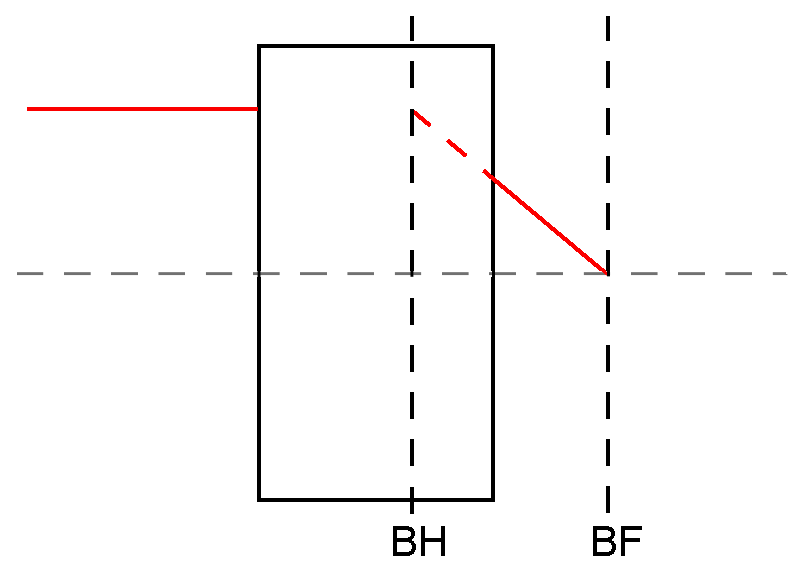
\includegraphics[scale=0.8]{./Images/optical_planes/optical_planes.eps}
	\caption{Illustration av bakra huvdudplan och fokalplan för ett godtyckligt optiskt system.}
	\label{fig:optical_planes}
\end{figure}

Lådan illustrerar ett optiskt system. Den röda strålen representerar strålgången. Det bakra fokalplanet, märkt BF, är planet där en parallell stråle skär den gråa centrallinjen och som är normalt på centrallinjen. Det bakra huvudplanet, märkt BG, är planet så att det optiska systemets verkan på strålan är ekvivalent med att all brytning sker i det planet, som illustrerat. Det fremre fokalplanet och huvudplanet fås på analogt sätt om man betraktar en stråle som kommer från höger.

\paragraph{Fokalavstånd}
Fokalavståndet till ett optisk system är avståndet från systemets bakre huvudplan till dets bakre fokalplan.

\paragraph{Konvexa och konkava linser}
En konvex linsa samlar parallela strålar, medan en konkav lins sprider parallella strålar.

\subsection{Ekvationer}

\paragraph{Reflektionslagen för plana speglar}
\begin{align*}
	s = -s'
\end{align*}
Alternativt, i kartesisk konvention:
\begin{align*}
	s = s'.
\end{align*}

\paragraph{Spegelekvationen för sfärisk spegel}
\begin{align*}
	\frac{1}{s} + \frac{1}{s'} = \frac{2}{R}
\end{align*}
Alternativt, i kartesisk konvention:
\begin{align*}
	-\frac{1}{s} + \frac{1}{s'} = \frac{2}{R}
\end{align*}
$R$ är spegelns krökningsradie.

\deriv

\paragraph{Brytning i sfäriska ytor}
\begin{align*}
	\frac{n_1}{s} + \frac{n_2}{s'} = \frac{n_2 - n_1}{R}
\end{align*}
Alternativ, i kartesisk konvention:
\begin{align*}
	-\frac{n_1}{s} + \frac{n_2}{s'} = \frac{n_2 - n_1}{R}.
\end{align*}

\deriv

\paragraph{Linsformeln för tunna linser}
\begin{align*}
	\frac{1}{s} + \frac{1}{s'} = \frac{1}{f}
\end{align*}

\deriv

\paragraph{Linsformeln för krökt lins}
\begin{align*}
	\frac{1}{s} + \frac{1}{s'} = \left(\frac{n_2}{n_1} - 1\right)\left(\frac{1}{R_1} - \frac{1}{R_2}\right)
\end{align*}

\section{Analytical Mechanics}

\paragraph{On the Handling of Constraints}
Suppose that the system moves under some constraint $g(x^{\mu}) = 0$. There are two ways to handle this.

The first is to introduce a Lagrange multiplier according to
\begin{align*}
	S = \integ{}{}{\theta}{\mathcal{L} + \lambda g}
\end{align*}
and extremize the action with the condition as an extra equation.

The other is to perform a coordinate transformation. Such transformations preserve the form of the equations of motion. The new coordinates are $q^{\mu}$ for all $\mu$ but the final one, and the final coordinate is $g$ itself. You can somehow then obtain equations of motion which can be solved by explicitly constraining $g$.

\paragraph{Constructing an Action}
To do analytical mechanics in a way that respects relativity, we will need an action. This will reasonably have to be constructed from some non-trivial Lorentz scalars. We try
\begin{align*}
	S = -\integ{}{}{\theta}{\sqrt{g_{\mu\nu}\dot{x}^{\mu}\dot{x}^{\nu}}m_{0}c + \frac{q}{c}\Phi_{\mu}\dot{x}^{\mu}},
\end{align*}
where we have parametrized the path in terms of some affine parameter. The involved quantities are the proper time and a line integral of the $4$-potential. The dots now signify derivatives with respect to this parameter. The equations of motion are
\begin{align*}
	\dv{\theta}\left(\frac{m_{0}c}{\sqrt{g_{\mu\nu}\dot{x}^{\mu}\dot{x}^{\nu}}}g_{\mu\nu}\dot{x}^{\nu} + \frac{q}{c}\Phi_{\mu}\right) - \frac{q}{c}\dot{x}^{\nu}\del{\mu}{\Phi_{\nu}} = 0.
\end{align*}

\paragraph{Reobtaining The Lorentz Force Law}
One way to proceed with the above is to choose $\theta = \tau$, for which we obtain
\begin{align*}
	\dv{\tau}\left(m_{0}g_{\mu\nu}\dot{x}^{\nu} + \frac{q}{c}\Phi_{\mu}\right) - \frac{q}{c}\dot{x}^{\nu}\del{\mu}{\Phi_{\nu}} = 0.
\end{align*}
Expanding the derivative yields
\begin{align*}
	m_{0}\ddot{x}_{\mu} = \frac{q}{c}\dot{x}^{\nu}\left(\del{\mu}{\Phi_{\nu}} - \del{\nu}{\Phi_{\mu}}\right) = \frac{q}{c}F_{\mu\nu}\dot{x}^{\nu},
\end{align*}
which is the expected equation of motion.

\paragraph{The Action and $3$-Vectors}
Another way to express the above is to choose $t$ as the parameter, whence the action becomes
\begin{align*}
	S = -\integ{}{}{t}{\sqrt{g_{\mu\nu}\dot{x}^{\mu}\dot{x}^{\nu}}m_{0}c + \frac{q}{c}(c\phi - c\vb{u}\cdot\vb{a})} = -\integ{}{}{t}{\sqrt{1 - \frac{\abs{\vb{u}}^{2}}{c^{2}}}m_{0}c^{2} + q(\phi - \vb{u}\cdot\vb{a})}.
\end{align*}
The corresponding generalized momentum is
\begin{align*}
	\vb{p} = -\frac{1}{2\sqrt{1 - \frac{\abs{\vb{u}}^{2}}{c^{2}}}}m_{0}c^{2}\cdot -\frac{2}{c^{2}}\vb{u} + q\vb{a} = \frac{1}{\sqrt{1 - \frac{\abs{\vb{u}}^{2}}{c^{2}}}}m_{0}\vb{u} + q\vb{a} = \gamma_{u}m_{0}\vb{u} + q\vb{a}.
\end{align*}
The equation of motion is
\begin{align*}
	\dv{t}(\gamma_{u}m_{0}\vb{u} + q\vb{a}) = -q\grad{\phi} + u_{j}\grad{a_{j}}.
\end{align*}
It can be shown that this is equivalent to
\begin{align*}
	\dv{t}(\gamma_{u}m_{0}\vb{u}) = q\vb{e} + q\vb{u}\times\vb{b}.
\end{align*}

\paragraph{A $3$-Vector Hamiltonian}
It can be shown from that the above that a corresponding Hamiltonian is
\begin{align*}
	\mathcal{H} = \sqrt{(m_{0}c^{2})^{2} + (\vb{p} - q\vb{a})^{2}c^{2}} + q\phi.
\end{align*}

\end{document}
